\chapter{Giới thiệu đề tài}
%\begin{large}  
\section{Đặt vấn đề}
\textit{Dữ liệu chuỗi thời gian} (time series data) là dữ liệu đo đạc được một cách tuần tự theo thời gian. Có rất nhiều loại dữ liệu có yếu tố thời gian như vậy, ví dụ như dữ liệu điện tâm đồ (ECG), dữ liệu thiên văn, thời tiết, mực nước, dữ liệu tài chính, giá chứng khoán… Một nghiên cứu khảo sát về các hướng nghiên cứu quan trọng và đang là thách thức trong lĩnh vực \textit{khai thác dữ liệu} (data mining) và \textit{học máy} (Machine Learning) được thực hiện vào năm 2006 bởi Yang và Wu \cite{st1} cho kết quả 10 hướng nghiên cứu chính. Trong đó, hướng nghiên cứu về khai phá dữ liệu chuỗi thời gian được xếp thứ 3 trong 10 hướng nghiên cứu quan trọng và thách thức nhất. Do đó, việc khai phá dữ liệu chuỗi thời gian đã và đang thu hút rất nhiều sự quan tâm nghiên cứu trên thế giới. Các bài toán tiêu biểu trong khai phá chuỗi dữ liệu thời gian bao gồm: \textit{Lập chỉ mục} (Indexing), \textit{Gom cụm} (Clustering), \textit{Phân tầng} (Classification), \textit{Tổng hợp} (Summarization), \textit{Phát hiện Motif} (Motif detection), \textit{Phát hiện chuỗi con bất thường} (Anomaly detection).

Khai phá dữ liệu chuỗi thời gian được ứng dụng rộng rãi trong nhiều lĩnh vực như y tế, kinh tế, tài chính, chứng khoáng, quản lý mạng truyền thông… Các lĩnh vực này thường cần độ chính xác cao. Trong khi đó, những \textit{chuỗi con bất thường} (anomalous subsequences) trên dữ liệu chuỗi thời gian thường ảnh hưởng rất nhiều đến kết quả khai phá dữ liệu. Hình \ref{fig:1-1} mô tả một chuỗi con bất thường trên đoạn dữ liệu điện tâm đồ (ECG).  Vì vậy, việc phát hiện chuỗi con bất thường trên dữ liệu chuỗi thời gian đóng vai trò rất quan trọng và thường được dùng như bước tiền xử lý cho những bài toán khai phá dữ liệu sau này. Sau đây là một vài ứng dụng quan trọng của bài toán phát hiện chuỗi con bất thường:

\begin{figure}[H]
    \centering
    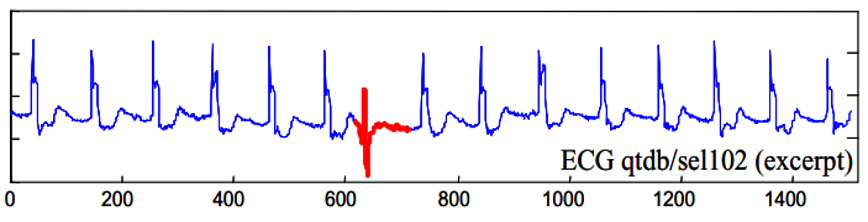
\includegraphics[scale=0.75]{./content/images/1-1.png}
    \caption{Chuỗi con bất thường trên dữ liệu điện tim đồ \cite{st12}}
    \label{fig:1-1}
\end{figure}

Phát hiện bất thường của xung nhịp tim trên dữ liệu điện tim đồ (ECG) \cite{st2} \cite{st12}: thông thường dữ liệu điện tim ECG là những chuỗi thời gian tuần hoàn ghi lại các biến thiên của các điện lực do tim phát ra trong hoạt động co. Một bất thường trong dữ liệu này có thể là một \textit{mẫu không phù hợp} (non-conforming pattern) về mặt chu kỳ hoặc biên độ, điều này chỉ ra rằng bệnh nhân có vấn đề về sức khoẻ.

Phát hiện bất thường của chuyến bay sử dụng dữ liệu cảm biến từ máy bay: hành vi hệ thống của chuyến bay được thể hiện bởi dữ liệu cảm biến thông qua các thông số khác nhau. Các thông số này có giá trị thay đổi trong suốt quá trình bay. Nếu dữ liệu cảm biến có chuỗi con bất thường thì có thể hành vi hệ thống chuyến bay đang có sai lệch, cần cảnh báo \cite{st3}.

Phát hiện tấn công trong các \textit{hệ thống tư vấn} (Recommender system): tấn công Shilling, trong đó kẻ tấn công đưa ra các xếp hạng, đánh giá có thiên vị để ảnh hưởng đến những kết quả tư vấn, gợi ý trong tương lai \cite{st4}.

Như vậy, phát hiện chuỗi con bất thường là một bài toán quan trọng, nhưng cũng nhiều thách thức trong dữ liệu chuỗi thời gian. Bởi vì dữ liệu đầu vào có thể chịu ảnh hưởng của nhiều yếu tố, dẫn đến sự không ổn định, hỗn loạn và có nhiều thành phần nhiễu (ví dụ như giá chứng khoán) \cite{st5}. Chính vì thế, không thể có một thông tin đầy đủ nào có thể biễu diễn chính xác mối quan hệ giữa giá trị tương lai với những giá trị trong quá khứ. Do đó, đối với bài toán phát hiện bất thường, các nhà nghiên cứu thường giả định rằng dữ liệu trong quá khứ có thể đại diện cho tất cả yếu tố tác động trong quá khứ, và dùng nó để dự đoán cho dữ liệu tương lai.

Trong thời gian gần đây, nhiều phương pháp phát hiện bất thường trong dữ liệu chuỗi thời gian đã được các nhà nghiên cứu áp dụng và mang lại hiệu quả trong các bài toán thực tế. Nổi bật trong số đó, có thể kể đến các phương pháp như: \textit{phương pháp dựa trên cửa sổ trượt} (sliding-window-based method), \textit{phương pháp dựa trên bài toán phân loại} (classification-based method), \textit{phương pháp dựa trên bài toán phân đoạn} (segmentation-based method). Gần đây nhất là \textit{phương pháp phát hiện bất thường dựa trên bài toán dự báo} (prediction-based method).

Đối với phương pháp phát hiện bất thường dựa trên bài toán dự báo, chúng ta có thể chia nó thành hai bài toán con. Thứ nhất là bài toán dự báo đối với dữ liệu chuỗi thời gian. Thứ hai là bài toán phát hiện bất thường dựa trên dữ liệu được dự báo.

Đi sâu vào bài toán dự báo dữ liệu chuỗi thời gian, nhiều năm trước, các nhà nghiên cứu đã sử dụng nhiều kỹ thuật tuyến tính để giải quyết bài toán này, một trong số đó là mô hình \textit{Auto-Regressive Intergrated Moving Average} (AMIRA) \cite{st6}. Vì đơn giản và phổ biến, nên phương pháp này thường được dùng để so sánh với các phương pháp hiện tại. Tuy nhiên, việc giả định chuỗi dữ liệu tuyến tính và không ổn định là không phù hợp với dữ liệu thực tế, vốn phi tuyến và hỗn loạn.

Với ưu điểm có thể mô hình hoá các dữ liệu phi tuyến, các mạng nơ-ron học sâu đã và đang thể hiện hiệu quả của mình trong các bài toán dự báo. Đầu tiên có thể kể đến \textit{mạng nơ-ron nhân tạo} (Artiticial Neural Networks - ANN). Nhiều nghiên cứu đã chứng minh rằng, ANN là một kỹ thuật hiệu quả để dự báo chuỗi dữ liệu thời gian. Tang và Fishwich \cite{st7fix}, Wang và Leu \cite{st8}, Jan và các cộng sự \cite{st9} đã chỉ ra rằng, ANN cho kết quả tốt hơn mô hình AMIRA, đặc biệt với dữ liệu không ổn định. Kết quả này có được là do khả năng mô hình hoá các hàm phi tuyến mà không cần bất cứ giả định nào của dữ liệu đầu vào. Bên cạnh đó, ANN cũng bộc lộ điểm yếu khi số lượng kết nối giữa các tầng quá lớn, dẫn đến trọng số của kiến trúc này nhiều. Điều này làm cho ANN không thể xây dựng được các mô hình phức tạp và dễ bị \textit{hiện tượng quá khớp} (overfitting) mà không thể làm tốt với dữ liệu ngoài thực tế.

Theo các giáo sư LeCun, Bengio và Hinton, \textit{học sâu} (deep learning) cho phép các mô hình tính toán gồm nhiều tầng xử lý để học biểu diễn dữ liệu với nhiều mức trừu tượng khác nhau \cite{st24}. Thời gian gần đây, học sâu dựa trên mạng nơ-ron nhân tạo (ANN) đang chứng minh được sự hiệu quả. Với việc sử dụng nhiều tầng nơ-ron, mạng nơ-ron học sâu đã biểu diễn dữ liệu tốt hơn so với các mạng truyền thống khác. Hình \ref{fig:1-2} mô tả một ví dụ về mạng nơ-ron nhân tạo có nhiều tầng.

\begin{figure}[H]
    \centering
    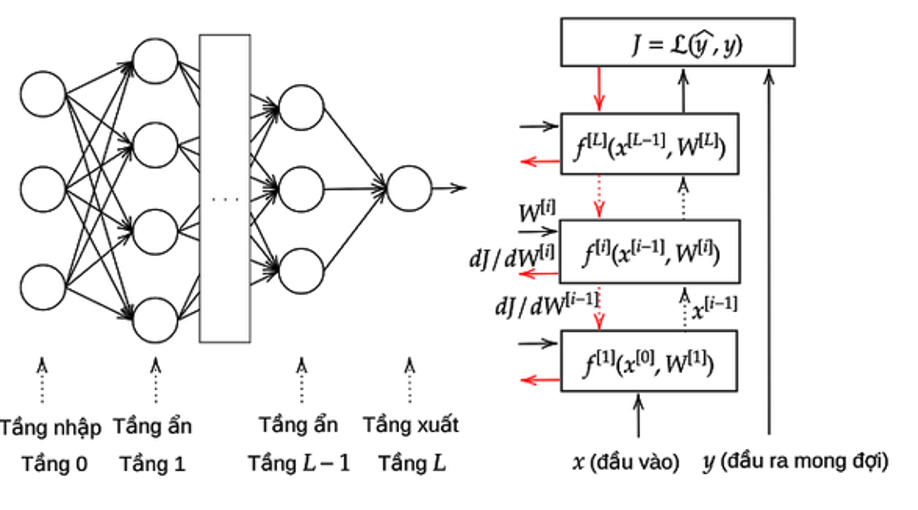
\includegraphics[scale=0.95]{./content/images/1-2.png}
    \caption{Một ví dụ về mạng nơ-ron nhân tạo nhiều tầng}
    \label{fig:1-2}
\end{figure}

Phần bên trái hình \ref{fig:1-2} cho thấy một mạng nơ-ron gồm nhiều tầng, trong đó nơ-ron của tầng trước \textit{kết nối đầy đủ} (fully-connected) với các nơ-ron của tầng sau. Mạng nơ-ron dạng này là \textit{mạng nơ-ron truyền thẳng} (Feed-forward Neural Networks – FNN) hay \textit{mạng perceptron nhiều tầng} (Multilayer Perceptron – MLP). Phần bên phải của hình \ref{fig:1-2} mô tả cơ chế lan truyền ngược để tính đạo hàm của hàm chi phí (hàm J) theo tham số ở từng tầng của mô hình.

Với kiến trúc độc đáo, \textit{mạng nơ-ron hồi quy} (Recurrent Neural Network - RNN) \cite{st10} \cite{st23} được biết đến nhiều trong các bài toán có dữ liệu chuỗi thời gian: dịch máy, chuyển giọng nói thành chữ và ngược lại, ECG, giá chứng khoán… Một điểm nổi bật của RNN chính là ý tưởng kết nối các thông tin phía trước để dự đoán cho hiện tại, các thông tin này khá gần với hiện tại. Nhưng, RNN lại thể hiện rõ khuyết điểm với dữ liệu có tính \textit{phụ thuộc xa} (long-term dependency), hay nói cách khác là dữ liệu tại thời điểm hiện tại chịu ảnh hưởng của dữ liệu khá lâu trong quá khứ. Như một điều tất yếu, mạng nơ-ron học sâu \textit{Long Short Time Memory} (LSTM) \cite{st11} xuất hiện như phiên bản nâng cấp của RNN, với sự kế thừa các ưu điểm của RNN, và giải quyết được vấn đề đối với dữ liệu có tính phụ thuộc xa trong mô hình RNN truyền thống.

Mạng nơ-ron học sâu LSTM được giới thiệu bởi Hochreiter và Schmidhuber (1997), và sau đó đã được cải tiến rất nhiều. Chúng hoạt động rất hiệu quả trên nhiều bài toán khác nhau nên dần đã trở nên phổ biến như hiện nay. Mạng nơ-ron học sâu LSTM được thiết kế để tránh được vấn đề phụ thuộc xa. 

Đi sâu vào bài toán con thứ hai, phát hiện bất thường là một trong những bài toán thú vị và đầy thách thức. Mỗi kiểu dữ liệu chúng ta lại có một phương pháp đặc thù để xác định bất thường. Từ thập niên 1980, các nhóm nghiên cứu đã đề xuất nhiều phương pháp phát hiện chuỗi bất thường trên dữ liệu chuỗi thời gian.

Nhìn chung, các phương pháp này dựa vào các kỹ thuật như: dùng xác suất thống kê đơn giản như \textit{Cu-Mulative Sum} (CUSUM) hoặc \textit{Exponentially Weighted Moving Average} (EWMA), hoặc phương pháp phát hiện bất thường dựa vào mật độ và khoảng cách. Bên cạnh đó cũng có các phương pháp đã được đề cập ở đầu chương như: phương pháp dựa vào cửa sổ trượt, sự tương tự, mô hình Markov ẩn, phân lớp hoặc phân đoạn. Các phương pháp này bộc lộ nhược điểm như: có nhiều loại bất thường trong dữ liệu, khó xác định độ dài chuỗi con, chuỗi thời gian kiểm thử và chuỗi thời gian huấn luyện có độ dài khác nhau, chuỗi thời gian trong thực tế thường dài và khi độ dài tăng thì độ phức tạp tính toán cũng tăng lên.

Trong nhóm phương pháp dựa vào cửa sổ trượt, có hai phương pháp để giải quyết bài toán phát hiện chuỗi con bất thường này được nhiều nhà nghiên cứu quan tâm và ưa chuộng, đó là giải thuật HOT SAX của Keogh và các cộng sự \cite{st12}, giải thuật WAT của Fu và các cộng sự \cite{st13}.

Một hướng đi khác, năm 2015, Malhotra và các cộng sự đã sử dụng ưu thế của mạng nơ-ron học sâu để giải quyết bài toán phát hiện bất thường \cite{st14}, bằng việc sử dụng mạng LSTM xếp chồng và sử dụng phân phối sai số dự báo để phát hiện bất thường. 

Bên cạnh đó, Buda và cộng sự đã kết hợp ưu thế của mạng nơ-ron học sâu, cũng như tính hiệu quả của mô hình AMIRA đối với dữ liệu tuyến tính và có tính ổn định để tăng hiệu quả cho bài toán dự báo, từ đó góp phần tăng độ chính xác cho bài toán dự báo \cite{st15}. 

\section{Mục tiêu nghiên cứu}
Với những tiềm năng đầy hứa hẹn của các mạng nơ-ron học sâu, trong nghiên cứu này chúng tôi sẽ áp dụng ưu thế của mạng nơ-ron học sâu trong bài toán dự báo, và dựa vào đó để phát hiện chuỗi con bất thường trên dữ liệu chuỗi thời gian. Để giải quyết được bài toán đề ra, chúng tôi sẽ xây mô hình học sâu, trọng tâm sử dụng mạng nơ-ron học sâu LSTM, vì các tập dữ liệu đều có sự tương quan giữa giá trị lịch sử tới giá trị hiện tại. Mặt khác, trong những năm gần đây, các nhà nghiên cứu đã sử dụng mạng nơ-ron học sâu LSTM trong các bài toán dự đoán giá trị của chuỗi thời gian và đạt kết quả tốt so với các kỹ thuật khác. Một bước tiến xa là các kết quả nghiên cứu này còn có thể được sử dụng trong các ứng dụng thực tế.

Kế thừa nghiên cứu của Malhotra và các cộng sự \cite{st14}, chúng tôi sẽ xây dựng mạng nơ-ron học sâu LSTM xếp chồng cho bài toán dự báo và sử dụng giải thuật phân phối sai số dự báo \cite{st16} cho bài toán phát hiện chuỗi con bất thường. Bên cạnh đó, kỹ thuật dự báo nhiều bước (multi-step ahead prediction) cũng sẽ được chúng tôi áp dụng để tăng tính hiệu quả cho chặng dự báo của công tác phát hiện bất thường \cite{st17}.

Nghiên cứu sẽ sử dụng những bộ dữ liệu mẫu từ các công trình đi trước. Những bộ dữ liệu này đã được đánh dấu chuỗi con bất thường. Nghiên cứu sẽ sử dụng những chuỗi con bất thường này để huấn luyện và đánh giá.

Ngoài ra, nghiên cứu cũng so sánh với giải thuật HOT SAX, một phương pháp nhận dạng chuỗi con bất thường được nhiều nhà nghiên cứu ưa chuộng. Chúng tôi sẽ so sánh về độ chính xác của các chuỗi con bất thường được phát hiện. Từ những kết luận rút ra được, chúng ta sẽ biết được phương pháp nào hiệu quả hơn trong công tác phát hiện chuỗi con bất thường trên dữ liệu chuỗi thời gian. Những điều này là những yếu tố quan trong khi sử dụng trong thực tế.

\section{Ý nghĩa đề tài}
Với nghiên cứu về phương pháp phát hiện bất thường bằng dự báo, đặc biệt là dựa vào ưu thế của mạng nơ-ron học sâu LSTM, đề tài có những ý nghĩa sau đây.

Ý nghĩa thực tiễn:
\begin{itemize}
\item Góp phần tìm ra tiềm năng của mạng nơ-ron học sâu LSTM trong khai phá dữ liệu chuỗi thời gian.
\item So sánh, đánh giá hiệu suất của phương pháp phát hiện bất thường bằng dự báo (mô hình để xuất) và phương pháp phát hiện bất thường bằng cửa sổ trượt (giải thuật HOTSAX).
\item Xây dựng được mô hình dự báo và phát hiện bất thường trên các bộ dữ liệu thuộc nhiều lĩnh vực.
\end{itemize}

%\newpage
Ý nghĩa khoa học:
\begin{itemize}
\item Góp phần đưa ra một mô hình, ứng dụng phương pháp học sâu vào bài toán phát hiện bất thường trên dữ liệu chuỗi thời gian.
\item Mở ra một hướng mới về phát hiện bất thường bằng dự báo dựa trên sự bùng nổ của phương pháp học sâu và mạng nơ-ron học sâu LSTM.
\end{itemize}

\section{Kết quả đạt được}
Trong nghiên cứu này, chúng tôi đề xuất mô hình dựa trên phương pháp phát hiện bất thường bằng dự báo để phát hiện bất thường trên các bộ dữ liệu thuộc nhiều lĩnh vực, đồng thời so sánh phương pháp này với phương pháp phát hiện bất thường dựa trên cửa sổ trượt, đại diện là giải thuật HOTSAX. Chúng tôi đề xuất xây dựng một mô hình dự báo có kiến trúc LSTM xếp chồng để tận dụng khả năng ghi nhớ thông tin của mạng nơ-ron học sâu LSTM.

Ngoài ra, chúng tôi sử dụng kỹ thuật dự báo nhiều bước để nâng cao khả năng dự báo của mô hình. Trong thực nghiệm, chúng tôi sử dụng 08 bộ dữ liệu thuộc nhiều lĩnh vực khác nhau để phát hiện bất thường, các bộ dữ liệu này đã được đánh dấu sẵn chuỗi con bất thường bởi các chuyên gia. Chúng tôi cài đặt mô hình đề xuất và giải thuật HOTSAX để tiến hành các kịch bản thực nghiệm, so sánh và đánh giá kết quả thực nghiệm trên các bộ dữ liệu này. Kết quả thực nghiệm cho thấy, mô hình đề xuất đã khắc phục được hạn chế của giải thuật HOTSAX khi dựa vào kích thước cửa sổ trượt. Nhưng bên cạnh đó, mô hình đề xuất cũng gặp phải nhiều cảnh báo sai đối với bộ dữ liệu có ít dữ liệu huấn luyện, do mô hình dự báo có nhiều sai số dự báo.

\section{Cấu trúc của luận văn}
Cấu trúc của báo cáo được tổ chức như sau:
\begin{itemize}
\item Chương 1 - Giới thiệu vấn đề: nhằm giới thiệu tổng quan về bái toán phát hiện bất thường dựa vào dự báo và phương pháp giải quyết.
\item Chương 2 - Cơ sở lý thuyết: trình bày những lý thuyết liên quan được sử dụng trong bài nghiên cứu.
\item Chương 3 - Các nghiên cứu liên quan: bao gồm các công trình nghiên cứu liên quan đến bài toán phát hiện bất thường, ứng dụng của bài toán phát hiện bất thường và các kỹ thuật dự báo nhiều bước trong chuỗi dữ liệu thời gian.
\item Chương 4 - Phương pháp nghiên cứu: phân tích đặc điểm của các bộ dữ liệu và trình cụ thể mô hình đề xuất và cách thức mô hình hoạt động. 
\item Chương 5 - Kết quả thực nghiệm: là kết quả đánh giá của mô hình đề xuất và so sánh với giải thuật HOTSAX 
\item Chương 6 - Kết luận: nêu ra các kết luận đúc kết được trong quá trình nghiên cứu và hướng phát triển tiếp theo trong tương lai. 
\end{itemize}
%\end{large}